\documentclass[tikz,border=2mm]{standalone}

\usepackage{amsmath}
\usepackage{helvet}
\renewcommand{\familydefault}{\sfdefault}

\usetikzlibrary{arrows.meta,calc,positioning}

% secondary text inside boxes (one \detail per line: \\ must not sit inside a group)
\newcommand{\detail}[1]{{\footnotesize\itshape #1}}

% ------------------------------------------------------------
% Colors (same families as the Bayesian-workflow figure)
% ------------------------------------------------------------
\definecolor{prepblue}{RGB}{0,112,192}
\definecolor{warmyellow}{RGB}{255,192,0}
\definecolor{collgreen}{RGB}{84,130,53}
\definecolor{anapurple}{RGB}{112,48,160}

\definecolor{preppanel}{RGB}{234,239,247}
\definecolor{warmpanel}{RGB}{253,249,237}
\definecolor{collpanel}{RGB}{245,246,244}
\definecolor{anapanel}{RGB}{243,239,248}

\definecolor{prepbox}{RGB}{203,216,238}
\definecolor{warmbox}{RGB}{255,239,193}
\definecolor{collbox}{RGB}{215,224,209}
\definecolor{anabox}{RGB}{225,214,238}

\definecolor{bordergray}{RGB}{89,89,89}
\definecolor{discardgray}{RGB}{150,150,150}

% Feedback colors
\definecolor{resample}{RGB}{190,100,0}    % re-tune / run longer  (short dash)
\definecolor{resampler}{RGB}{0,112,192}   % change sampler         (long dash)

\begin{document}

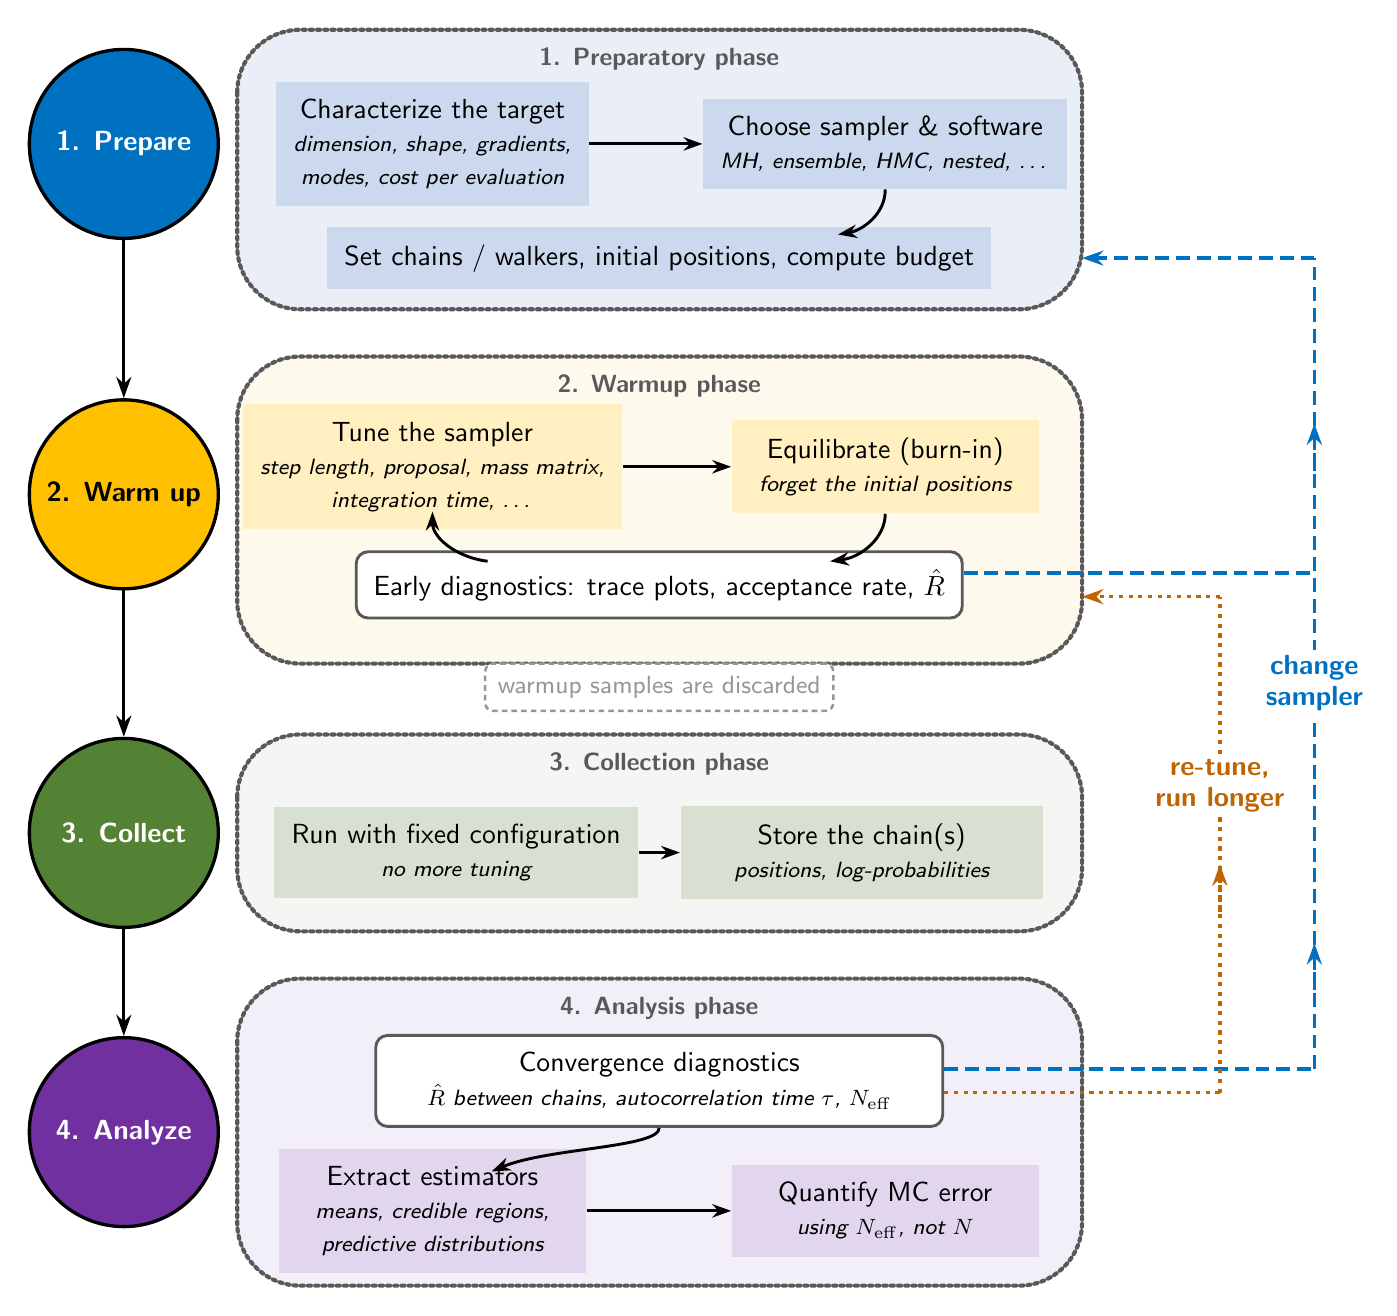
\begin{tikzpicture}[
    x=1cm,
    y=-1cm,
    font={\sffamily\fontsize{10pt}{12pt}\selectfont},
    flow/.style={
        draw=black,
        line width=1.15pt,
        -{Stealth[length=2.7mm,width=1.9mm]}
    },
    cycle/.style={
        draw=black,
        line width=1.05pt,
        -{Stealth[length=2.4mm,width=1.7mm]}
    },
    panel/.style={
        draw=bordergray,
        fill=#1,
        line width=1.5pt,
        dash pattern=on 1.1pt off 1.5pt,
        line cap=round,
        rounded corners=8mm
    },
    phase/.style 2 args={
        circle,
        draw=black,
        fill=#1,
        line width=1.2pt,
        minimum size=2.40cm,
        text=#2,
        align=center,
        font=\bfseries\sffamily\fontsize{10pt}{11pt}\selectfont
    },
    box/.style={
        fill=#1,
        draw=none,
        align=center,
        inner sep=2.2mm
    },
    panellabel/.style={
        font=\bfseries\sffamily\fontsize{9.5pt}{11pt}\selectfont,
        text=bordergray
    },
    diag/.style={
        draw=bordergray,
        fill=white,
        line width=1.05pt,
        rounded corners=1.5mm,
        align=center,
        inner sep=2.2mm
    },
    discard/.style={
        draw=discardgray,
        fill=white,
        text=discardgray,
        line width=0.9pt,
        dash pattern=on 2pt off 1.5pt,
        rounded corners=1mm,
        align=center,
        inner sep=1.6mm,
        font=\sffamily\fontsize{9pt}{10pt}\selectfont
    },
    discardarrow/.style={
        draw=discardgray,
        line width=0.9pt,
        dash pattern=on 2pt off 1.5pt,
        -{Stealth[length=2.2mm,width=1.6mm]}
    },
    fbtune/.style={
        draw=resample,
        line width=1.25pt,
        dash pattern=on 1.5pt off 2.0pt
    },
    fbsampler/.style={
        draw=resampler,
        line width=1.25pt,
        dash pattern=on 5pt off 2.5pt
    },
    fbtunearrow/.style={fbtune,-{Stealth[length=2.7mm,width=1.9mm]}},
    fbsamplerarrow/.style={fbsampler,-{Stealth[length=2.7mm,width=1.9mm]}},
    fbtunelabel/.style={
        font=\sffamily\bfseries\fontsize{10pt}{11pt}\selectfont,
        text=resample, fill=white, align=center, inner sep=2pt
    },
    fbsamplerlabel/.style={
        font=\sffamily\bfseries\fontsize{10pt}{11pt}\selectfont,
        text=resampler, fill=white, align=center, inner sep=2pt
    }
]

% ============================================================
% LEFT-HAND PHASE SEQUENCE
% ============================================================
\node[phase={prepblue}{white}]   (prep) at (1.23, 1.75) {1. Prepare};
\node[phase={warmyellow}{black}] (warm) at (1.23, 6.20) {2. Warm up};
\node[phase={collgreen}{white}]  (coll) at (1.23,10.50) {3. Collect};
\node[phase={anapurple}{white}]   (ana)  at (1.23,14.30) {4. Analyze};

\draw[flow] (prep.south) -- (warm.north);
\draw[flow] (warm.south) -- (coll.north);
\draw[flow] (coll.south) -- (ana.north);

% ============================================================
% 1. PREPARATORY PHASE
% ============================================================
\draw[panel=preppanel] (2.67,0.30) rectangle (13.40,3.85);

\node[panellabel] at (8.03,0.68) {1. Preparatory phase};

\node[box=prepbox, minimum width=3.9cm, minimum height=1.05cm] (p1) at (5.15,1.75)
{Characterize the target\\\detail{dimension, shape, gradients,}\\\detail{modes, cost per evaluation}};

\node[box=prepbox, minimum width=3.9cm, minimum height=1.05cm] (p2) at (10.90,1.75)
{Choose sampler \& software\\\detail{MH, ensemble, HMC, nested, \dots}};

\node[box=prepbox, minimum width=7.6cm, minimum height=0.60cm] (p3) at (8.03,3.20)
{Set chains / walkers, initial positions, compute budget};

\draw[cycle] (p1.east) -- (p2.west);
\draw[cycle] (p2.south) .. controls (10.90,2.65) and (10.60,2.85) .. (10.30,2.90);

% ============================================================
% 2. WARMUP PHASE
% ============================================================
\draw[panel=warmpanel] (2.67,4.45) rectangle (13.40,8.35);

\node[panellabel] at (8.03,4.83) {2. Warmup phase};

\node[box=warmbox, minimum width=3.9cm, minimum height=1.05cm] (w1) at (5.15,5.85)
{Tune the sampler\\\detail{step length, proposal, mass matrix,}\\\detail{integration time, \dots}};

\node[box=warmbox, minimum width=3.9cm, minimum height=1.05cm] (w2) at (10.90,5.85)
{Equilibrate (burn-in)\\\detail{forget the initial positions}};

\node[diag, minimum width=6.4cm, minimum height=0.60cm] (w3) at (8.03,7.35)
{Early diagnostics: trace plots, acceptance rate, $\hat R$};

\draw[cycle] (w1.east) -- (w2.west);
\draw[cycle] (w2.south) .. controls (10.90,6.75) and (10.60,7.00) .. (10.20,7.05);
\draw[cycle] (5.85,7.05) .. controls (5.45,7.00) and (5.15,6.75) .. (5.15,6.42);

% warmup samples are discarded
\node[discard] (bin) at (8.03,8.65) {warmup samples are discarded};

% ============================================================
% 3. COLLECTION PHASE
% ============================================================
\draw[panel=collpanel] (2.67,9.25) rectangle (13.40,11.75);

\node[panellabel] at (8.03,9.63) {3. Collection phase};

\node[box=collbox, minimum width=4.6cm, minimum height=0.95cm] (c1) at (5.45,10.75)
{Run with fixed configuration\\\detail{no more tuning}};

\node[box=collbox, minimum width=4.6cm, minimum height=0.95cm] (c2) at (10.60,10.75)
{Store the chain(s)\\\detail{positions, log-probabilities}};

\draw[cycle] (c1.east) -- (c2.west);

% ============================================================
% 4. ANALYSIS PHASE
% ============================================================
\draw[panel=anapanel] (2.67,12.35) rectangle (13.40,16.25);

\node[panellabel] at (8.03,12.73) {4. Analysis phase};

\node[diag, minimum width=7.2cm, minimum height=0.95cm] (a1) at (8.03,13.65)
{Convergence diagnostics\\{\footnotesize\itshape $\hat R$ between chains, autocorrelation time $\tau$, $N_\mathrm{eff}$}};

\node[box=anabox, minimum width=3.9cm, minimum height=1.05cm] (a2) at (5.15,15.30)
{Extract estimators\\\detail{means, credible regions,}\\\detail{predictive distributions}};

\node[box=anabox, minimum width=3.9cm, minimum height=1.05cm] (a3) at (10.90,15.30)
{Quantify MC error\\{\footnotesize\itshape using $N_\mathrm{eff}$, not $N$}};

\draw[cycle] (a1.south) .. controls (8.03,14.50) and (6.60,14.50) .. (5.90,14.80);
\draw[cycle] (a2.east) -- (a3.west);

% ============================================================
% FEEDBACK TRACKS
%  inner (orange, short dash): re-tune / run longer -> warmup
%  outer (blue,  long  dash):  change sampler       -> preparatory
% ============================================================
\coordinate (tunebusbottom)    at ([yshift=-1.5mm]a1.east -| 15.15,0);
\coordinate (tunebustop)       at (15.15,7.50);
\coordinate (samplerbusbottom) at ([yshift= 1.5mm]a1.east -| 16.35,0);
\coordinate (samplerbustop)    at (16.35,3.20);

% from analysis diagnostics
\draw[fbtune]    ([yshift=-1.5mm]a1.east) -- ([yshift=-1.5mm]a1.east -| tunebusbottom);
\draw[fbsampler] ([yshift= 1.5mm]a1.east) -- ([yshift= 1.5mm]a1.east -| samplerbusbottom);
% from warmup diagnostics (change sampler only)
\draw[fbsampler] ([yshift=1.5mm]w3.east) -- ([yshift=1.5mm]w3.east -| samplerbusbottom);

% inner track
\draw[fbtune] (tunebusbottom) -- (tunebustop);
\draw[fbtunearrow] (15.15,11.50) -- (15.15,10.90);
\node[fbtunelabel] at (15.15,9.90) {re-tune,\\run longer};
\draw[fbtunearrow] (tunebustop) -- (13.40,7.50);

% outer track
\draw[fbsampler] (samplerbusbottom) -- (samplerbustop);
\draw[fbsamplerarrow] (16.35,12.50) -- (16.35,11.90);
\draw[fbsamplerarrow] (16.35,5.90) -- (16.35,5.30);
\node[fbsamplerlabel] at (16.35,8.60) {change\\sampler};
\draw[fbsamplerarrow] (samplerbustop) -- (13.40,3.20);

\end{tikzpicture}

\end{document}
